\chapter{Introduction}

\begin{itemize}
    \item Get the audience to identify with someone or something, - Give that someone or something some kind of need, - And start changing the circumstances.
    \item Have that someone or something deal with the new circumstances - And find the thing that was needed.
    \item Have that someone or something pay the price of the find - And start heading back toward the original circumstances.
    \item show how those original circumstances have changed as a result.
\end{itemize}
\emph{Dan Harmon's story telling circle}


\section{The Research}
Software app developers need to deliver software that can be used successfully by end users. To do so they need to be able to create software and distribute it so it is available to end users. End users need to be able to install and use that software. If the software is sufficiently usable, useful and behaves adequately they may continue to use it. Developers cannot assess \emph{a priori} whether their software will meet the needs and expectations of users, meet their needs, or the needs of their stakeholders. In short they do not know whether it will thrive.

One of the key considerations is whether the quality of their apps are adequate. There are many ways to assess quality of apps, including static analysis, in-person testing, and automated testing. Users may perform their own subjective assessments of quality and some of these users provide feedback in the form of ratings and reviews. 

Researchers have investigated these various sources of quality related information. My research concentrates on using sources of analytics related to usage of apps to help developers a) assess the quality of their current software, and b) improve the quality using the same analytics sources.

This research was inspired by learning about the power and capabilities of applying usage data collected by mobile apps in extremely popular real-world mobile apps in the early days of mobile apps (before Android, iOS and other modern mobile platforms were released). At the time I worked for Google and was responsible for testing all Google's mobile apps, including: Search, GMail, Maps, and many others.

Several years later, when consulting with another company with over ten million active users I discovered they had included two analytics tools in their apps where there were numerous discrepancies in the data collected, the ways the counted and the resulting reports, yet they were both considered necessary. The engineers then added a third analytics library in the hope it would correlate with one or other of the existing libraries - it didn't, instead it had distinct characteristics and counts. And yet the developers were able to discover how their apps were used in incredible detail and by applying what they learned their apps became increasingly popular and financially successful.

These experiences led me to starting my PhD in order to research the potential of mobile analytics, and to understand some of their flaws and the effects of those flaws. During my research there have been incredible changes in the mobile landscape (for instance major manufacturers, operating systems, etc. have appeared, mushroomed, and disappeared). Similarly many test automation tools and frameworks have been and gone. Meanwhile, apps and app stores have spread beyond smartphones and tablets to desktop operating systems, cloud-based product offerings such as Salesforce, etc. Google's Android platform includes platform-level data collection, reporting and analytics intended to help developers learn about ways they can improve their apps. Meanwhile regulation has started to emphasise and highlight some of the many risks and concerns with gathering data wantonly. 

Despite all these changes, and my limited inroads into a subset of the entire landscape, the research seems to indicate the potential of applying usage analytics to improve both the product (the software) and the process (how the software is developed and tested). The research also identified flaws within analytics tools and also between analytics tools. Both the potential and the flaws appear worth sharing with researchers and with practitioners to help them chose and use analytics wisely.


\subsection{Research Problem}
Research into the use and efficacy of software usage analytics appears to be under-served, particularly in terms of being able to use the analytics to identify and potentially address quality flaws in apps in use. And in recent years, platform-wide analytics has been made available to all the developers of actively used Android apps in Google Play. Despite the ubiquity of these platform-level analytics there appeared to be no research into their efficacy, completeness, or accuracy.


\subsection{Research Contributions}
The research presents the results of several case studies in the use of analytics to improve the reliability of a variety of mobile apps.

TBC.

\subsection{Research Scope}
Developers have various sources of feedback about their apps, as Figure~\ref{fig:sources-of-feedback-for-developers} illustrates. The pink triangle represents the extent of Google Play (the app store) in terms of providing feedback. Other feedback is also available independently of the app store, for instance by using software incorporated directly into the app and from the development process.

\begin{figure}[ht]
    \centering
    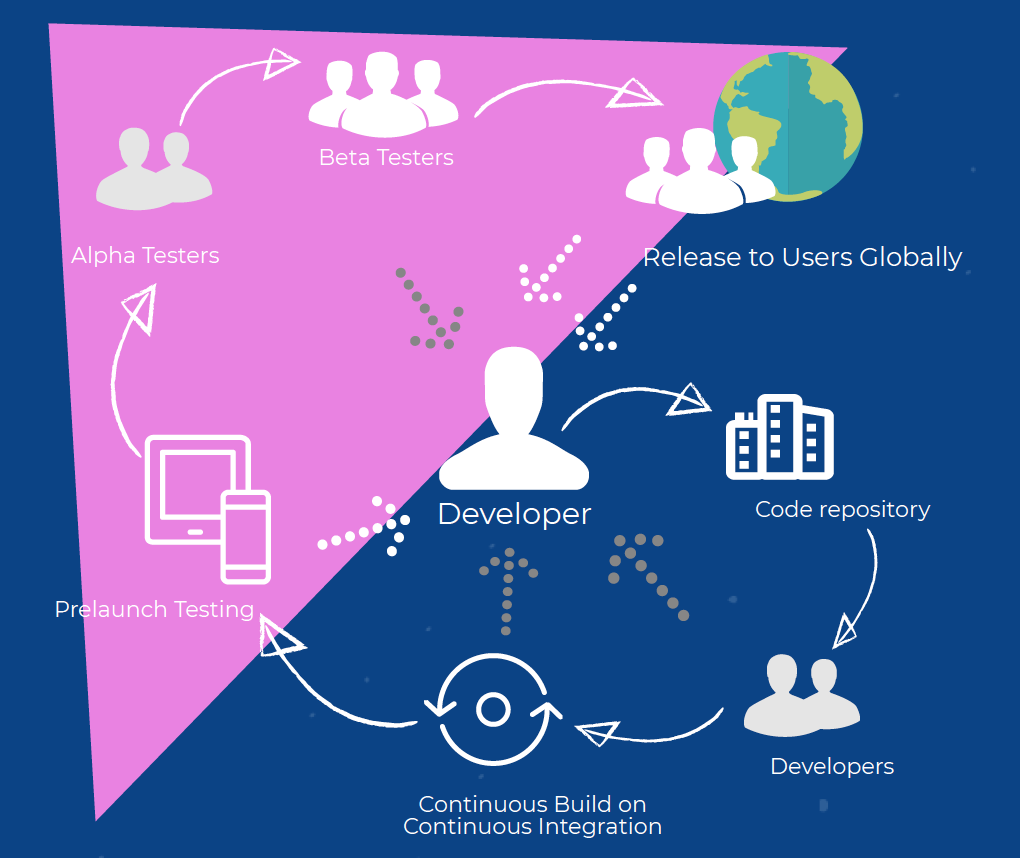
\includegraphics[width=13cm]{images/silvias-developer-centric-figure-mobilesoft2020.png}
    \caption{Sources of feedback for developers}
    \label{fig:sources-of-feedback-for-developers}
\end{figure}

Each source of feedback may stem from humans (for example, in reviews) or from software (for example, from code quality tools such as Lint). This research introduces three sources of software generated feedback.

\subsection{Research Strategy}


\section{Findings}\label{findings-section}
The application of mobile analytics has enabled each of the development teams who participated in the research to materially improve their measured reliability. 

For the first case study the reliability was improved approximately 12x for the main Kiwix Android application by applying the approach identified in this research. 
During the initial improvement stages the reliability of the project's custom apps did not improve. These custom apps are built using the main application's source code, and when the improved codebase was used to create new releases of the custom apps their reliability also improved several fold.

\begin{figure}[ht]
    \centering
    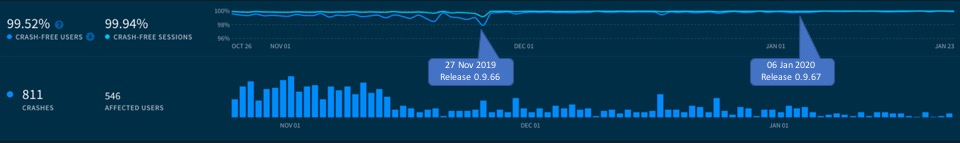
\includegraphics[width=\textwidth]{images/annotated_pocketcode_90_day_fabric_crashlytics_report.jpg}
    \caption{Pocket Code improvements in crash rate, in 90 days}
    %\Description{Pocket Code: When the project team investigated crashes they improved the reliability}
    \label{fig:pocketcode_improvements_in_crash_rate}
\end{figure}

An unacceptably high crash rate for the key Pocket Code Android app were tamed within two releases and 7 weeks by applying the approach described in this thesis. The changes needed to make the improvements were small. Figure \ref{fig:pocketcode_improvements_in_crash_rate} shows the improvement in crash rate as measured by Fabric Crashlytics. When the experiment started the crash rate was nearly four times the maximum threshold recommended by Google in their Android Vitals service and the project team had not been able to address the crash rate despite applying many of the recognised and recommended software development practices over several years~\cite{adamsen2015systematic_catrobat, luhana2018streamlining, ali2019behavior_catrobat, ali2019using_catrobat, hirsch2019approach_catrobat, schranz2019contributors_catrobat, slany2014tinkering}.

The developers continue to actively use mobile analytics to highlight potential quality issues and address pertinent issues promptly. One of the project teams chose to add an additional analytics tool to both their Android and iOS apps with the objective of improving the teams understanding of broader quality concerns. These quality concerns now also include usability. The team aims to use the data to improve the usability and user experience for their current and future users. They are designing the analytics to retain and protect user privacy, both important and highly relevant concerns.

Mobile Analytics can be incorporated as additional sources of information for development teams in harmony with other sources of information - it is not exclusive or exhaustive.

The analytics tools Google provides to developers of Android apps in Google Play Console have value despite the many flaws my research uncovered in their tools and reports. Some are mentioned in published papers~\cite{harty_google_play_console_insightful_development_using_android_vitals_and_pre_launch_reports, harty_better_android_apps_using_android_vitals, harty_improving_app_quality_despite_flawed_mobile_analytics}, the current known set are in this thesis. The research identified major differences in the reports and analytics provided by two analytics tools from the same company. There were both internal and cross-tool flaws and inconsistencies. Some of these have already been reported to Google in preparation for a full report to be submitted on completion of some ongoing research.

Fully automated pre-launch reports are effective at finding some quality flaws in Android apps at no financial cost and minimal effort by the app developers. These reports are provided by the app store and intended to help developers identify quality issues with their Android apps in order to address these issues so they do not affect end-users.

\subsection{The following section to be revised and moved}

 

Google Play uses data collected automatically from users opted-in to provide usage and diagnostics data to Google. The data is collected at a per-device level, which means that one device could potentially report data from several user accounts, conversely for users who use multiple devices some may provide the data while others do not.


I instigated and led the development of several opensource software utilities to help record and preserve reports and underlying failure data from Google Play Console and Android Vitals. We have successfully extended the capabilities of the utilities and further extensions are practical. Research benefits:
\begin{itemize}
    \item Evidence preserved for analysis:
    \item Data can now be compared and further assessed:
    \item Data and contents can be shared by developers of Android apps with other researchers - extending the body of knowledge about crashes (un-reliability) and ANRs (run-time unresponsiveness). \emph{bringing previously unknown data, practices and tools into the open so others can understand them, make more informed decisions, and perform further research.}
\end{itemize}

I made data available~\cite{harty_wama_dataset_examples} for further research based on data originally only made available to app developers. Larger volumes of data are available upon request.

The research has been presented at various conferences and workshops, including at NII Shonan in 2019 at meeting 152 on "Release Engineering for Mobile Applications"~\footnote{~\url{https://shonan.nii.ac.jp/seminars/152/}}. 

\section{Outline of this thesis}
Bugs are ubiquitous in software (even one of the most respected software engineers, Donald E. Knuth, recognises, publicly acknowledges, \emph{and pays for}~\cite{knuth_trutex, wikipedia__knuth_reward_checks_2020} bugs found in his creations. And self-aware developers expect there will be bugs in their software. \emph{``You are entitled to a reward of at least 0x$1.00 ($2.56) if you are the first person to report a bona-fide error not on those lists."} Donald E. Knuth~\cite{knuth_the_bank_of_san_serriffe}

Even top development teams are likely to learn of bugs they were not able to find, and cannot reproduce. For instance, Google's Android Auto Team have asked for help from end users to identify patterns that may help the team find and address a long-running and frustrating bug in Android Auto~\footnote{\url{https://support.google.com/androidauto/thread/2865341?msgid=44437416}}. As reported by \texttt{autoevolution} in May 2020:  
\emph{"As it turns out, the Android Auto team wasn’t able to reproduce the whole thing, so it’s now asking users to send additional reports with more information to help fix the problem."}~\footnote{~\url{https://www.autoevolution.com/news/google-wants-users-to-help-fix-widespread-android-auto-bug-143760.html}}.


\subsection{Validation of the concepts}
My practical research focuses on two sets of Android applications, those of the Kiwix and Catrobat project teams. According to data and reports Google provides the development teams their active user-bases are 362,595 for the Kiwix project across 18 published apps, and 148,966 for the Catrobat project across 6 published apps. %data obtained on 16th May 2020.
TODO map these apps to the buckets in the table from the 'beyond Google Play' paper.

While these apps include a useful variety of user populations (from 10's of users to 150K+ across many countries and tens of apps) they could be perceived as a \emph{drop in the ocean} of the millions of apps currently available in the Google Play app store. Also, both project teams are non commercial, and may have different working dynamics from commercial development projects and teams. As my research was inspired from my consulting work with businesses who rely on the success of their apps I chose to supplement these two projects by engaging with developers from several commercial development teams. These include: Moonpig, Moodspace, and LocalHalo. Each values and uses analytics data during their development process to assess post-launch issues with their apps. From time to time things go awry with the behaviours of one or more of their releases and analytics helps them to identify and respond to issues before they become pervasive. For the LocalHalo app, \emph{TODO add details}... For Moonpig \emph{TODO add details}...

\subsubsection{Validation by the Google Engineering Team}
In Spring 2019 I reported various flaws or potential anomalies in various reports Google Play Console provides to developers to the then Product Manager for Android Vitals, Mr Fergus Hurley. As the long-term product owner he has extensive and insider experience of the tools and reports Google provides to an estimated population of over 1 million Android developers \emph{TODO add references e.g. to the Beyond Google Play paper and the one about a few developers creating an exponential number of apps}. I asked for his perspective during both a long in-person meeting and a follow-up video call a few weeks later. He confirmed several of the issues and debated others. He was willing to go on record in one of my accepted peer-reviewed papers on the topic \emph{TODO add link} and asked me to continue to share my findings with them. During the next 12 months he and then they added more Google staff to the discussion and asked me to write up my findings in a document that became over 30 pages long. Their policy means they are unlikely to confirm changes they make as a result of my research and findings, nonetheless they accept and value the feedback that has been provided. They also confirmed various bugs were ones they want to address.
